\documentclass{article}

% --- load packages ---
\usepackage[margin=1in]{geometry} % change the margins
\usepackage{amsmath} % useful math environments and commands like align
\usepackage[colorlinks,bookmarks,bookmarksnumbered,allcolors=blue]{hyperref} % hyperlinks between references
\usepackage[justification=centering]{caption}
\usepackage{graphicx}  % include images
\usepackage[table,xcdraw]{xcolor}
%\usepackage[caption=false]{subfig} % subfigures.  false option prevents conflicts in caption styling with other packages
\usepackage{booktabs} % better tables
\usepackage[capitalise]{cleveref} % better referencing. uses cref.
\usepackage[section]{placeins} % sometimes useful to prevent figures from floating out of a section
\usepackage{cite} % handles multiple citations in one command better
\usepackage{doi} % allow correct hypderlinking of DOIs
\usepackage[normalem]{ulem}
%\usepackage{float}git pu
\usepackage{pdfpages}
\usepackage{tikz}
\usepackage{csvsimple}
\usepackage{adjustbox, lipsum}
\usepackage{setspace}
\usepackage{minted}
\usepackage{epstopdf}
\usepackage{subcaption}
\usetikzlibrary{tikzmark}

\useunder{\uline}{\ul}{}
\newcommand{\wide}{0.7\linewidth}
%\epstopdfDeclareGraphicsRule{.pdf}{png}{.png}{convert #1 \OutputFile}
%\epstopdfDeclareGraphicsRule{.eps}{png}{.png}{convert #1 \OutputFile}
%\DeclareGraphicsExtensions{.png,.pdf}


\begin{document}
\singlespacing
\title{HW \#2 Surrogate Modeling}
\author{Landon Wright}
% put in \date{} if you don't want a date to appear, or enter a specific date, otherwise default is today's date.
\maketitle
\section{Implementation Discussion}
% Chosen parameters

% Solution

% Algorithm performance

% comparison to expectations
  % 10 runs from different points
% How decided on max perturbation

% Were you able to tune so that it reliably solved the problem

% average number of function evaluations to reach optimum

\subsection{Convergence paths}
% path to convergence for at least three different starting points

\subsection{Matlab Implementation}
\inputminted[xleftmargin=10pt, linenos]{matlab}{simAnneal.m}
\end{document}
%\begin{table}[t]
%	\begin{center}
%		\caption{Values of the model output variables.}
%		\label{tab:outmaxmin}
%		\noindent\adjustbox{max width=\textwidth}{%
%			\csvautotabular{OutBounds.csv}}
%	\end{center}
%\end{table}
%
%
%\begin{figure}[h]
%	\centering
%	\includegraphics[width=\wide]{Profiler}
%	\caption{Profiler showing the pridicted outputs from the inputs}
%	\label{fig:profiler}
%\end{figure}

% \subsection{Forward Difference Implementation}\label{sec:fd_code}
%\inputminted[xleftmargin=10pt,linenos]{matlab}{fd_obj_grad.m}

%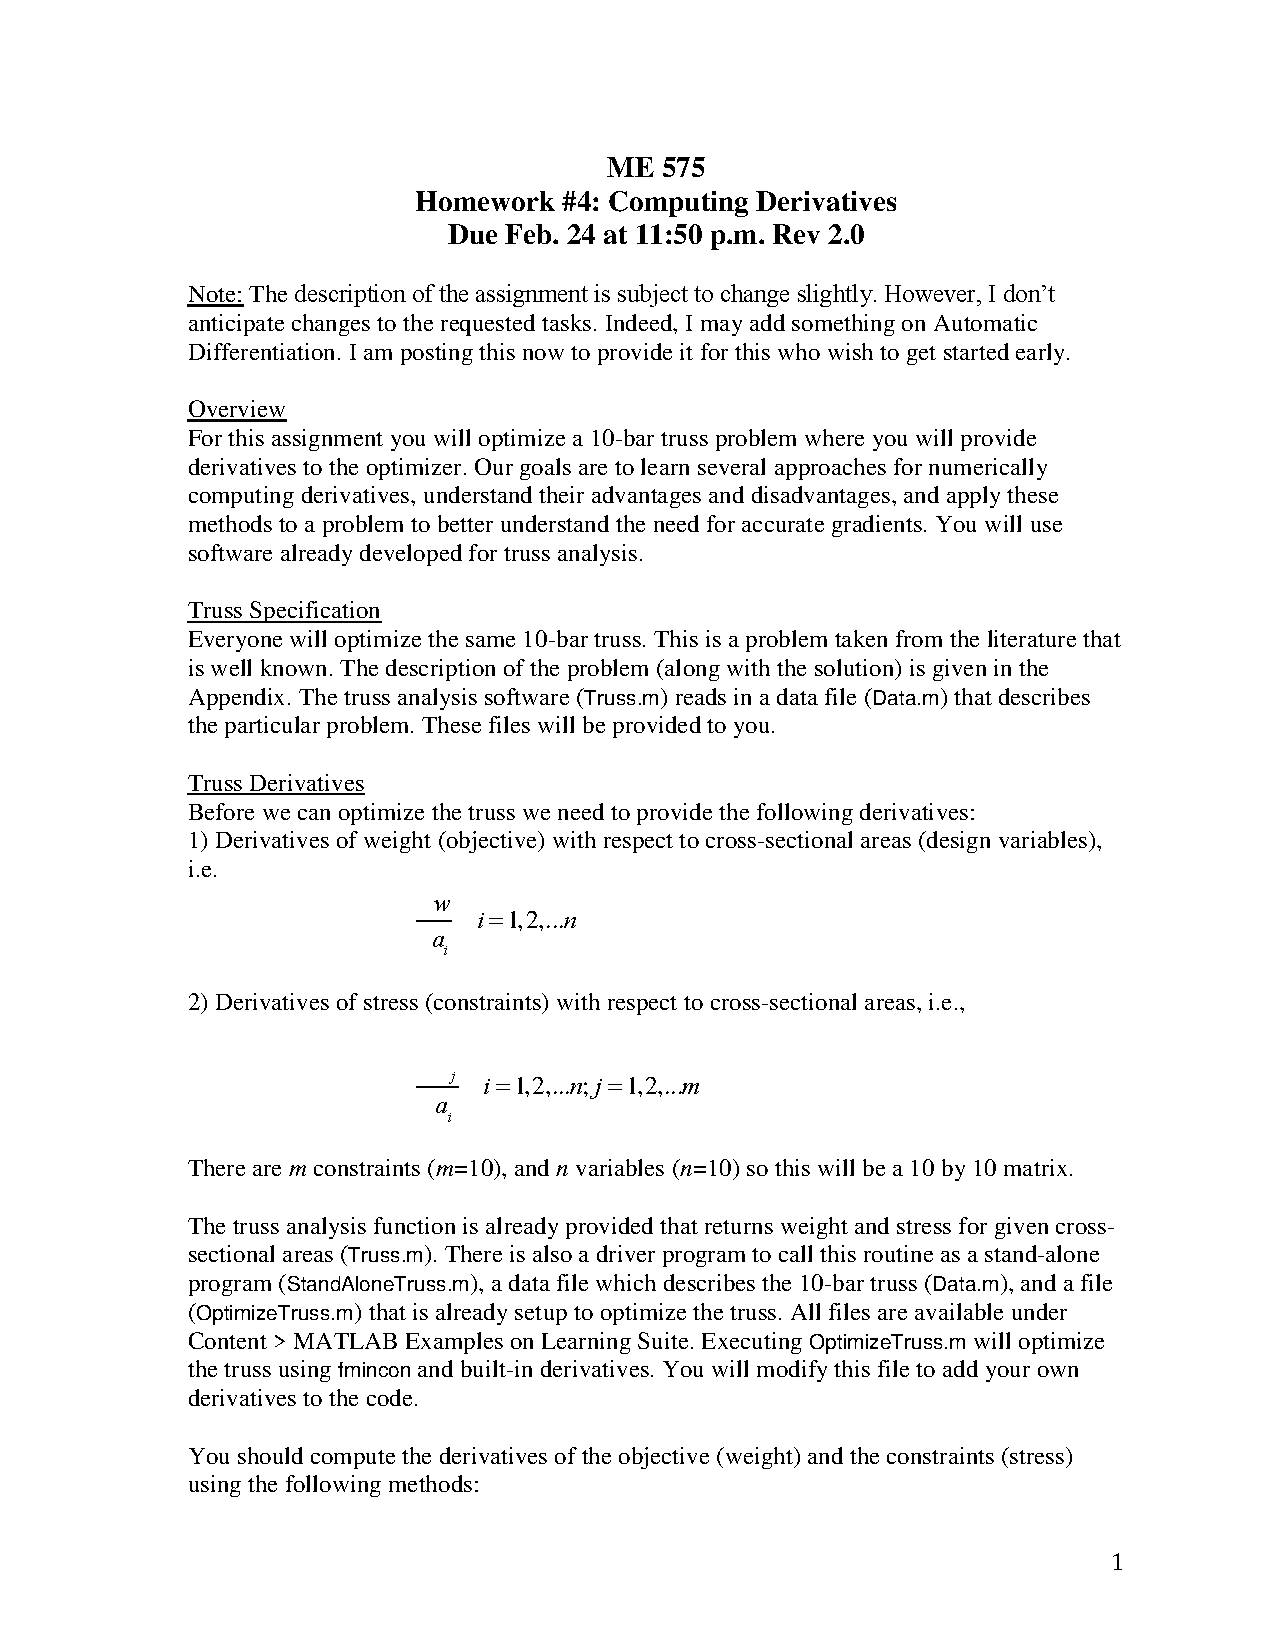
\includepdf[pages=-, pagecommand={}]{HW4.pdf}
